\chapter{Approach}

After reviewing early cognitive studies on expert performance, we present this study of systematic literature review which explores the current practice of expertise location in Software Engineering. First we illustrate the approach and protocol to conduct the review. This review is based on guidelines provided by \citeauthor{KITCHENHAM20132049} \cite{KITCHENHAM20132049}. In following sections, we specify the goals for each research question, and then provide the six-step-process in details for our review, the keywords and domains for literature searching queries: the list of literature searching engines, the standard for conference filtering, and finally the evaluation matrices for literature.

\section{Research Questions}

There are different types of experts in the field of software engineering practices. When organizers or managers intend to maximize the benefit of specific domain experts for their teams, they need to understand the expertise of each member in the group. In order to understand the capability of an organization, one of the most intuitive and efficient way is locating experts from their previous experience \cite{mcdonald2000expertise}. Due to the popularity of online open source communities, we expect to employ more data sources to generate suggestion for locating different types of experts through rich public activity data. In this study, we survey the nature of expertise in the field of software engineering, and another goal is to review approaches from state-of-the-art expertise location research. Therefore, we purpose the following two main research questions:\\

\fbox{\begin{minipage}{\linewidth}
\textbf{RQ1}: In the field of Software Engineering, what are the measurable characteristics that distinguish experts from novices or less-experienced subjects?
\end{minipage}}
\hfill\break
By answering the first research question, we target to conclude the characteristics that differentiate experts from less-experienced and novice developers. In addition to studies included in background section, we also expect to learn through surveyed studies to find if there were other criteria to identify expert developer.\\

\fbox{\begin{minipage}{\linewidth}
\textbf{RQ2}: How do state-of-the-art expertise/expert location approaches and systems compile these characteristics and then locate expertise?
\end{minipage}}
\hfill\break
From the second the research question, we intend to investigate data sources and expertise models that each study adopted to determine their experts under various sub-domains. However, there are various and complex sub-domains under software engineering. When searching for various expertise location methods, we intend to examine if the model can be applied to OSS community, or if OSS public data could contribute to improve the locating quality (e.g., precision and recall) while additional public data can be included.

Through answering these two research questions, we expect to summarize the approaches for locating different types of expertise/experts in software engineering, and provide directions to design future expertise location systems which enable the tremendous public dataset from OSS and knowledge sharing sites. Further, use these expert as role models to guide novice software developer for their careers \cite{STEINMACHER201567}.

\section{Literature Survey Framework}

Our literature search approach is inspired by following literature survey studies in software \cite{STEINMACHER201567, Fathy2018Large}. Before starting the research process, we set up the targeting publication venues. In order to ensure the focus and quality of the literature that we are studying for constructing the initial sample, we filter out the conferences and journals other than A ranks according to ERA\footnote{http://libguides.newcastle.edu.au/researchimpact/eralist}, Qualis\footnote{http://www.capes.gov.br/} and CCF\footnote{http://history.ccf.org.cn/sites/paiming/2015ccfmulu.pdf} these three rankings systems. In addition to the initial searching process, and we performed one round of citation searching (snowball sampling) after we constructed the initial sample. Further, at the end of sample construction, we manually added several relevant literature to our literature repository.

The overall literature selection process is as following:

\begin{enumerate}
\item Searching digital libraries: we queried digital libraries, and then store the query result at a local paper repository which is managed by a free and open sour-source reference management tool, Zotero\footnote{https://www.zotero.org}, and it manages bibliographic data of the paper and also related copies of the paper, such as PDF files. Moreover, we uses their chrome extension, Zotero Connector\footnote{https://chrome.google.com/webstore/detail/zotero-connector/ekhagklcjbdpajgpjgmbionohlpdbjgc?hl=en} to transfer the search result from web to the local paper repository.
\item Title, abstract and keywords filtering: since our query contains several generic terms in the domain of software engineering, the searching result is not promising in recall. We perform a first level of filtering on title, abstract and keywords to check if the studies is relevant to our major objectives based on meta-data to reduce the cost of the study. From this step, we exclude most irrelevant papers to our research questions.
\item Introduction and conclusion analysis: then we analyze the starting and ending sections of the literature to identify their primary research goals and contribution. This part of analysis could enable us to one step further to valid whether the purpose of the subject is relevant to our research questions.
\item Citation search: for studies found relevant after all previous steps, we conduct search on through Google Scholar which aggregates literature across different resources. Then we perform the same analysis on meta-data, introduction and conclusion to decide whether to include these studies. At this step, we dismiss the filter of Rank A conference, but include literature from all other publication venues as long as the paper is relevant to the objective.
\item Manual addition: we also include a few studies that have promising contribution to this field, especially answering our research question but not covered by the query result at the end of the study. 
\item Full literature reading: at last, if a paper is included after all previous steps, we perform a comprehensive reading throughout the paper, but also decide whether to exclude the literature in the last step.

\end{enumerate}

\begin{figure}
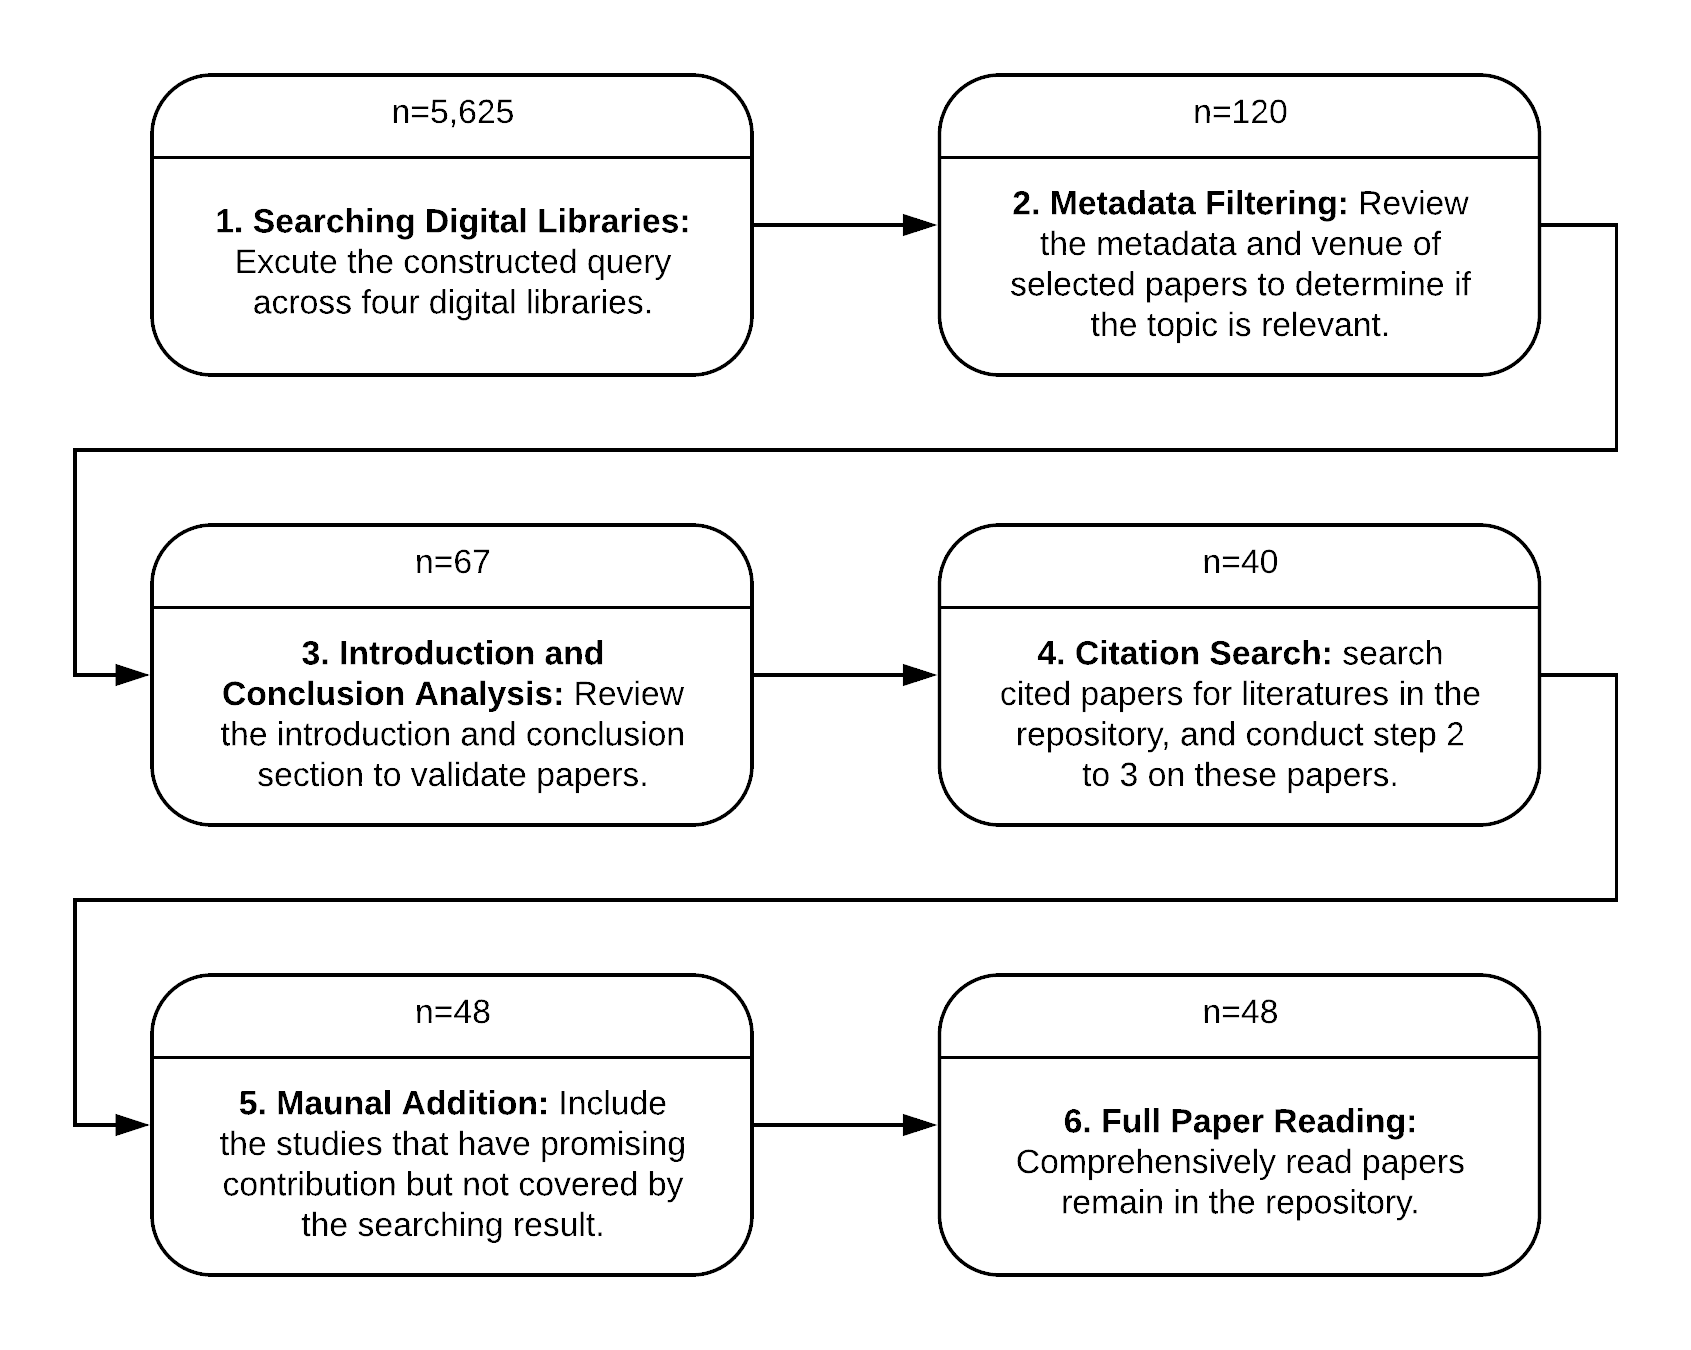
\includegraphics[width = \columnwidth]{process}
  \caption{Literature Selection Process}
  \label{fig:process}
\end{figure}

According to our research questions, we restrict our studying fields with the range of Software Engineering, Human-Computer Interaction, and Computer Supported Collaborative Work. By limiting the conferences that we are studying, we not only limited our research focuses based on RQs, but also exclude papers that are not in English or not published in a peer-reviewed venue. As a result, based three publication venue ranking systems that we referred, the rank A conferences under these categories are: ICSE, FSE, ASE, CSCW and CHI; the rank A journals are: IJHCS, TOCHI, TOSEM, TSE, and CSCW.

\begin{table}[tbp]
\centering
\begin{tabular}{l l}
\hline
\textbf{Item}      & {\textbf{Keyword}}                              \\ \hline
Domain I  & software, system, program          \\ 
Domain II & development, develop, engineer       \\ 
Expertise & expertise, expert, skill, knowledge \\ \hline
\end{tabular}
\caption{Keywords for Constructing the Searching Query}
\label{table:keyword}
\end{table}

We determine keywords that we would include to perform the literature search (see Table \ref{table:keyword}) upon RQ1 and RQ2. The keyword list has two major fields that we are interested in this study: domain of software engineering, and expertise location. The first set of keywords (Domain I) indicates software artifact is the subject that we are concerning and its synonyms. The second the set of keywords (Domain II) indicates that we are interested in expertise involved in the production procedure of software. The last set of the keywords contain the main subject of this study, expertise, and its synonyms.

Query based textual search expression is the most available and effective mechanism to retrieve literature through digital libraries. Based on the keywords in the Table \ref{table:keyword}, we constructed a searching query connected by binary operators, which is supported by most literature search engines (see Figure \ref{fig:query}). 

\begin{figure}
\begin{verbatim}
{
  ("software" OR "system" OR "program") 
  AND 
  ("development" OR "develop" OR "engineer") 
  AND 
  ("expertise" OR "expert" OR "skill" OR "knowledge" OR "ability" OR 
  "talent")
}
\end{verbatim}
  \caption{Query Performed for Searching Literature}
  \label{fig:query}
\end{figure}

After determining the query, we select digital libraries to conduct the search. Our selection criteria are based on following: It should include major publication venue in Software Engineering, HCI, and CSCW in English, support binary operators in queries, and provide full paper access. Therefore, we selected four digital libraries to conduct our search: ACM Digital Library \footnote{https://dl.acm.org/}, IEEE Digital Library \footnote{https://ieeexplore.ieee.org/}, Scopus \footnote{https://www.scopus.com/}, and Springer \footnote{https://link.springer.com/}.

\begin{table}[tbp]
\centering
\begin{tabular}{l l}
\hline
\textbf{Conference} & \textbf{Searching Results} \\ \hline
CSCW       & 278               \\ 
ICSE       & 1451              \\ 
CHI        & 2224              \\ 
ASE        & 84                \\
FSE        & 70                \\ \hline
\end{tabular}
\caption{Searching Result of Conference Publications}
\label{table:searching_conf}
\end{table}

\begin{table}[tbp]
\centering
\begin{tabular}{ll}
\hline
\textbf{Journal} & \textbf{Searching Results} \\ \hline
CSCW    & 505               \\
IJHCS   & 811               \\ 
TOCHI   & 69                \\
TOSEM   & 92                \\
TSE     & 41                \\ \hline
\end{tabular}
\caption{Searching Result of Journal Publications}
\label{table:searching_jour}
\end{table}

\section{Literature Sampling}

\textbf{Searching Digital Libraries}: We used the query presented in Section 3.1 to retrieve an initial sample of papers, which was executed on Mar 19, 2018 across four digital libraries, and results are ordered by relevance according to each digital library.  also used the Rank A conferences in Section 3.1 as a filter to limit result amount. See the amount initial literature sample in the table filtering by title and abstract. All queries are performed on meta-data indexing of the literature for consistency (The meta-data of a paper includes its title, abstract, and keywords).  See Table \ref{table:searching_conf} and \ref{table:searching_jour} for initial sample by publication venue from aggregated searching result. Noticeably, since we employs a reference management software to manage our paper repository and bibliographic data, it automatically to filter the duplicates of papers as we transfer the searching results into the repository in the software. Thus, there is no such a phase in our approach that removes the duplicates.

\begin{table}[tbp]
\centering
\begin{tabular}{ll}
\hline
\textbf{Conference} & \textbf{Initial Sample} \\ \hline
CSCW       & 12             \\ 
ICSE       & 39             \\ 
CHI        & 15             \\ 
ASE        & 10             \\ 
FSE        & 6              \\ \hline
\end{tabular}
\caption{Amount of Papers for Each Conference Venue in the Initial Sample}
\label{table:sample1_conf}
\end{table}

\begin{table}[tbp]
\centering
\begin{tabular}{ll}
\hline
\textbf{Journal} & \textbf{Initial Sample} \\ \hline
CSCW       & 10             \\ 
IJHCS       & 15             \\ 
TOCHI        & 1             \\ 
TOSEM        & 4             \\ 
TSE        & 8              \\ \hline
\end{tabular}
\caption{Amount of Papers for Each Journal Venue in the Initial Sample}
\label{table:sample1_jour}
\end{table}

\textbf{Meta-data Filtering}: Then based on the searching result, a researcher manually inspects the meta-data of each result to determine whether the literature is relevant to the topic. At this phase, we exclude papers that not focus on software, e.g., expertise sharing over a medical team, papers on expert systems, papers of keynote speeches and presentation notes, and also duplication. As a result, we generates an initial sample of 120 candidate papers from 5 conference venues and also 5 journal venues. See Table \ref{table:sample1_conf} and \ref{table:sample1_jour} for numerical details by venues.

\textbf{Introduction and Conclusion Analysis}: In this step, we focus on the research method, contribution and application of studies include. We exclude 53 papers which are not fitting our objectives in the research questions, for reasons such as: observational study without purposing method/tool, or a study on exploring expertise in software production but without providing approach to locate it.

\textbf{Citation Search}: After previous step, we conduct one level of citation search (snowball sampling) on papers in the repository. We are particularly focus on studies conducted by authors already in the repositories, and researches with high impact (high volume of citation count provided by Google Scholar). We initially relied on the citation counts from the original digital library where paper was found, but the result is not promising as original library may lack of counting citations from publication venues are not included in this library, or even not providing a counting number. Therefore, we apply Google Scholar to search the paper again, and use the citation count provided by the system to determine our initial and very brief assessment on research impact. From this step, we include another 6 studies into our paper repository, and also we do not filter papers from publication venue standard that we used at the second step.

\textbf{Manual Addition}: There are a few important studies that are not covered by our searching query, neither could not be reflected through snowball sampling. At the end of the sample construction process, we manually add a few studies that have promising research objectives, or provide directional future plans in the field according to expert recommendation. These studies are most aggregating data across multiple collaboration sites. We will provide detailed analysis in the result section.

\textbf{Full Paper Reading}: In the last step of sampling process, we start our analysis process while still be open to exclude studies that not focus on our research questions. As a result, we did not exclude any papers at this stage. In the following section, we will provide the evaluation matrices that we adopted during full paper reading process. 

\section{Evaluation Matrices}

\begin{table}[tbp]
\resizebox{\columnwidth}{!}{%
\centering
\begin{tabular}{lll}
\hline
\textbf{Item}                               & \textbf{Purpose}  & \textbf{Definition}                                                                                        \\ \hline
Title                              & Overview & What is the title of the literature?                                                               \\ 
Year                               & Overview & When did the literature publish?                                                                   \\ 
Publication 
Venue                  & Overview & Where did the literature publish?                                                                  \\ 
Publication 
Type                   & Overview & What is the type of the literature (journal, conference, demo, or book)?                          \\ 
Authors                            & Overview & Who are the authors of the literature?                                                             \\ 
Research 
Type                      & Overview & What is the research approach of the literature (empirical, case study or conceptual)?            \\ 
Expertise 
Domain                   & RQ1, RQ2 & Which domain can the expertise being apply to? Software coding/testing/design etc?                \\ 
Expertise 
Model                    & RQ1, RQ2  & What is the mathematics or theoretical model of the expertise?                                      \\ 
Theory base & RQ1      & Are there any theoretical background for this model (e.g., from cognitive science/engineering/novel)? \\ 
Memory 
Engagement                  & RQ1      & Does the expertise model reflect any memory engagement associating with expertise?                \\ 
Application of Studies             & RQ2      & How does the expertise/expert location system improve the field of software engineering?          \\ 
Granularity          & RQ1, RQ2 & What is the granularity of the expertise model (element/method/file/project)?                          \\ 
Future Work             & Direction      & What is future work of this study, particularly on expertise location?                             \\ \hline
\end{tabular}
}
\caption{Evaluation Matrices for Reviewing Papers}
\label{table:evaluation}
\end{table}

While conducting full paper reading, we setup the evaluation matrices to collect items that we are concerned according to our research question. We listed following 13 items extracted from each literature in our paper repository (See Table \ref{table:evaluation}).

\textbf{Research overview}: There are 6 items in this category. We included the meta-data of the publication in this category like title, year, publication venue, publication type, authors and research type, especially authors of research which used for extracting primary studies in later sections. In addition to meta-data, we also identify the research types (\textit{e.g.,} conceptual, empirical, case study, ethnographic \textit{etc}.) for each paper that we reviewed. Therefore, we could summarize the suitable research methods for specific research questions in expertise studies.

\textbf{Expertise Domain}: As we mentioned in the background section 2.3, software engineering is complex subject with multiple sub-domains. Through collecting expertise domain, we intend to investigate the status of expertise location techniques in a specific area, for example, bug report assignment, merging conflict resolution, and software fault location. We also intend to look for if there is any area that does not have approach to locate expertise.

\textbf{Expertise Model}: We use this item to capture the conceptual or mathematical model for locating expertise. For example, Servant and Jones \cite{servant2012whosefault} use a mathematical model of \textit{speciousness} of a fault and \textit{recency} of changes on a specific line of code to determine the expertise of a developer to fix a bug. Further, an expertise model can also be represented by a very high level conceptual model such as \cite{Ye2002Supporting} uses a four-layer model to classify knowledge and expertise of functionality in application. We intend to summarize approaches to locate, or even quantify expertise for software engineers in a certain domain.

\textbf{Theory Base}: We also intend to collect any theory base behind the expertise model that each study adopted. The theory can be purposed within the study based on author's suggestion, or a field study conducted before, or referred from engineering or management literature. Theory bases evince the expertise model that adopted by these studies, and  are applicable for larger scale.

\textbf{Memory Engagement}: Based on multiple research that were referred in the background chapter, the cognitive expertise for software engineering task is rooted in developer's long-term memory. From this item, we intend to investigate the long-term memory reflection of expertise models, \textit{i.e.,} whether an expert determined by an expertise model was capable of reflecting information processing ability such as recalling more related memory for the subject.

\textbf{Application}: This item focuses on the application and contribution of this study. We collect this item mostly according to authors suggestion and proposal in their paper, which are usually represented in the introduction, discussion, and conclusion sections. Through summarizing this item, we intend to explore our views on implications for expertise location techniques in software engineering, such as in hiring, training, and etc..

\textbf{Granularity}: The granularity of the study mainly focuses the scale of expertise could be reflected by the model. If an expertise model utilizes the methods level coding behavior to assign developer for implementing a program method, then this model would be not applicable to determine this developer's overall knowledge on the project which contains the method. 

\textbf{Future work}: Suggestions on future work or directions can usually be found in discussion and conclusion sections based on preference of the authors. Despite the fact that each study has its own very different purpose, from this survey, we aim to analyze and summarize the suggestions from each sub-domains, and overlook a high level future direction of expertise location approaches. 

We analyze papers in our literature repository based on the evaluation matrices listed above but not limited to. There are several cases that some of the item is not applicable to a particular study, but the overall the evaluation matrices is actionable for majority of the studies in the paper repository.